\documentclass[11pt,openany]{book}
\usepackage{geometry}
\geometry{
	letterpaper
}
\usepackage{blindtext}
\usepackage{tikz,tcolorbox}
\usepackage{pgfplots}
\usepackage{xcolor}
\usepackage{amsfonts}
\usepackage{hyperref} 
\usepackage{indentfirst}
\usepackage{graphicx}
\usepackage{caption}
\usepackage{subcaption}
\usepackage[normalem]{ulem}
\usepackage [english]{babel}
\usepackage [autostyle, english = american]{csquotes}
\usepackage{appendix}
\usepackage{tabularx}
\usepackage{amsmath,amssymb}
\usepackage{mathtools}
\usepackage{makecell}
\graphicspath{ {./images/} }
\usepackage{enumitem}
\usepackage{soul}
\usepackage{mathtools}
\usepackage{wrapfig}
\usepackage{mathrsfs}
\usepackage{centernot}
\usepackage{amsthm}
\usepackage{listings}
%\usepackage{biblatex}
%\addbibresource{bibliograph.bib}
\usepackage{microtype}
\usepackage{pagenote}


\definecolor{codegreen}{rgb}{0,0.6,0}
\definecolor{codegray}{rgb}{0.5,0.5,0.5}
\definecolor{codepurple}{rgb}{0.58,0,0.82}
\definecolor{backcolour}{rgb}{0.95,0.95,0.92}

\lstdefinestyle{mystyle}{
	backgroundcolor=\color{backcolour},   
	commentstyle=\color{codegreen},
	keywordstyle=\color{magenta},
	numberstyle=\tiny\color{codegray},
	stringstyle=\color{codepurple},
	basicstyle=\ttfamily\footnotesize,
	breakatwhitespace=false,         
	breaklines=true,                 
	captionpos=b,                    
	keepspaces=true,                 
	numbers=left,                    
	numbersep=5pt,                  
	showspaces=false,                
	showstringspaces=false,
	showtabs=false,                  
	tabsize=2
}

\lstset{style=mystyle}
%% End notes to be printed as sections at the
%% end of each chapter.
\renewcommand*{\notedivision}{\section*{\notesname}}
\renewcommand*{\pagenotesubhead}[1]{}

%\newcommand*{\exercises}{\section*{\exercisename}}
%%%%%%%%%%%%% For customising the endnote markers. Comment these out if you don't want them.
% To prefix each note number with the chapter number
\renewcommand{\thepagenote}{\thechapter-\arabic{pagenote}}

% To have a slightly different formatting for the endnote numbers in the text -- smaller text, sans-serif, square brackets
\renewcommand\notenumintext[1]{\space{\footnotesize\sffamily[FN-#1]}}

% To have a slightly different formatting for the endnote numbers in the notes section. Just the square brackets and sans-serif; normal size.
\renewcommand\notenuminnotes[1]{{\sffamily[FN-#1] }}
% If you want a different name/heading for the end notes
\renewcommand{\notesname}{End Notes}
\newcommand{\exercisename}{Exercises}
\newcounter{exercisecounter} % continuity of exercises in a section
\newenvironment{exerciselist}{
	\begin{enumerate}
		\setcounter{enumi}{\value{exercisecounter}}
	}{
		\setcounter{exercisecounter}{\value{enumi}}
	\end{enumerate}
}
\newcommand*{\exercises}{\section*{\exercisename}}

%%%%%%%%%%%%% End customisation
\newcommand{\reals}{\mathbb{R}}
\newcommand\defeq{\mathrel{\stackrel{\makebox[0pt]{\mbox{\normalfont\tiny def}}}{=}}}

\newcounter{thmcounter} % continuity of theorem
\newcommand{\definition}[2]{\begin{tcolorbox}[title=Definition {\thechapter}.{\arabic{thmcounter}} ({#1}),colframe=black,label={def:\thechapter.\thethmcounter}]
		{#2}\end{tcolorbox}

\addtocounter{thmcounter}{1}
}
\newcommand{\proposition}[1]{\begin{tcolorbox}[title=Proposition {\thechapter}.{\arabic{thmcounter}},colframe=red!50!blue!20!white,colback=red!35!blue!10!white, coltitle=black,label={prop:\thechapter.\thethmcounter}]{#1}\end{tcolorbox}
\addtocounter{thmcounter}{1}
}
\newcommand{\theorem}[2]{\begin{tcolorbox}[title=Theorem {\thechapter}.{\arabic{thmcounter}} ({#1}),colframe=red!70!black,colback=red!5!white,label={thm:\thechapter.\thethmcounter}]{#2}\end{tcolorbox}
	
	\addtocounter{thmcounter}{1}
}
\newcommand{\example}[1]{\begin{tcolorbox}[title=Example {\thechapter}.{\arabic{thmcounter}},colframe=yellow!50!white,colback=yellow!20!white,coltitle=black,label={ex:\thechapter.\thethmcounter}]{#1}\end{tcolorbox}

\addtocounter{thmcounter}{1}
}
\newcommand{\corollary}[1]{\begin{tcolorbox}[]{Corollary {\thechapter}.{\arabic{thmcounter}}: {#1}}\end{tcolorbox}
	
	\addtocounter{thmcounter}{1}
}
\newtheorem*{remark}{Remark}
\newtheorem*{notation}{Notation}
%\newcommand{\exercises}{\section*{\exercisename}}
%% THIS LINE IS MANDATORY
\makepagenote

\begin{document}
	\tableofcontents
	% sample chapter
	\iffalse
	\chapter*{Sample chapter}
	\setcounter{thmcounter}{1}
	\section*{Section}
	This is a sample chapter structure.\\
	\definition{Real numbers}{
		We denote $\mathbb{R}$ as the set of real numbers. Intuitively, this set contains all the "decimals" including the non-terminating ones.
	}
	\theorem{Cantor}{
		The cardinality $|\mathbb{R}|$ is larger than $|\mathbb{Z}|$.
	}
	\begin{proof}
		Left as an exercise.
	\end{proof}
	\corollary{
		There is no bijective function mapping $\mathbb{Q}$ to $\mathbb{R}$.
	}
	\begin{proof}
		There is a bijective function from $\mathbb{Z}$ to $\mathbb{Q}$.
	\end{proof}
	\example{
		$1.3$ is a real number. So we say $1.3 \in \mathbb{R}$. \\
		$\pi$ is a real number. So we say $\pi \in \mathbb{R}$.
	}

	\exercisename

	\begin{enumerate}
		\item Show that all the zeros of $\zeta(s)$ lie on the line $\Re (z)=1/2$.
	\end{enumerate}
	\fi
	\chapter{Coordinate Geometry}
\setcounter{exercisecounter}{0}

\setcounter{thmcounter}{0}
\section{Introduction}
Many of you have encountered some form of coordinate geometry in high school. For instance, the ``standard" way to visualize a graph e.g. $f(x)=x^2$ is to visualize the points in 2-D space $(x,y)$ where $y=x^2$. We give a demonstration in Python code.

\begin{lstlisting}[language=Python]
import matplotlib.pyplot as plt
import numpy as np
X=np.arange(-100,100) #create list of numbers from -100 to 100
Y= X**2 #calculate the square of at each x
plt.plot(X,Y) #plot all the pairs of points in 2d plane
plt.xlabel('x')
plt.ylabel('y=x^2')
plt.title('Visualization of the "object"')
plt.show()
plt.show()
\end{lstlisting}
\begin{tikzpicture}
	\node (A) at (0,0) {$x$};
	\node (B) at (3,0) {$x^2$};
	\draw[->,thick]
	(A)--(B)
	node[midway,below] {the ``graph" object} ;
	\node(whitehead) at (8,0){
		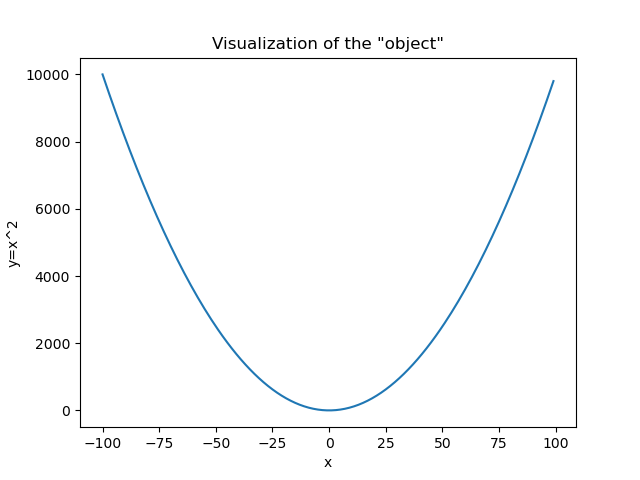
\includegraphics[width=0.6\textwidth]{coordinate_geometry/square_graph.png}
	};
\end{tikzpicture}


This is also known as the Cartesian plane, named after René Descartes who invented it in the 17th century.\\
\section{Visualization of geometric objects}

The Cartesian plane allows us to describe shapes with equations and perform calculations with them. We first define the playing field (the Cartesian plane and higher dimensional analogues) and the players.
\definition{Real numbers}{
	The set of \textbf{real numbers}, denoted as $\mathbb{R}$, is (informally) the set of all the numbers that can be written out in decimal form.
}
\example{
The following are real numbers:
\begin{enumerate}
	\item The integers $0$, $\pm 1$, $\pm 2$, ...  
	\item Fractions in the form $\frac{a}{b}$, where $a$ and $b\neq 0$ are integers.
	\item Irrational numbers $\sqrt{2}$, $\pi$.
\end{enumerate}
}
\begin{remark}
	The set of real numbers is known as a \textbf{complete field}. The definition of a complete field will be swept under the rug, but it guarantees a few things. The most important property: We will not ``escape" the set by performing operations, possibly infinitely many.
\end{remark}
\definition{N-dimensional space}{
	Let $n$ be a positive integer. We denote the \textbf{n-dimensional real space} to be $\mathbb{R}^n$, consisting of all the $n$-tuples $(x_1,x_2,x_3,...,x_n)$, where each $x_j$ is a real number. \\
	We call an $n$-tuple $(x_1,...,x_n)$ a \textbf{point}, and two points $(x_1,...,x_n)$ and $(y_1,...,y_n)$ are equal if $x_j=y_j$ for all $j$-th entries of the tuples.
}
\begin{remark}
	We sometimes use $\mathbf{x}$ to denote $(x_1,...,x_n)$ to make notation cleaner.
\end{remark}
\subsection{Lines}
Now that we have introduced the playing field of n-dimensional space, we can start translating the axioms of euclidean geometry to this coordinate system.
\definition{Lines}{
	In euclidean geometry, a line is defined by two points. We let $\mathbf{x},\mathbf{y} \in \mathbb{R}^n$. The \textbf{line} going from $\mathbf{x}$ to $\mathbf{y}$ is denoted $\overrightarrow{\mathbf{xy}}$.
}
What would this line look like? To get from $\mathbf{x}$ to $\mathbf{y}$, we have to traverse $y_1-x_1$ units in the first coordinate, $y_2-x_2$ units in the second, ..., $y_n-x_n$ in the last. We thus have a natural notation for the line $\overrightarrow{\mathbf{xy}}$.
\[
 \overrightarrow{\mathbf{xy}}=(y_1-x_1,y_2-x_2,...,y_n-x_n).
\]

This is very similar to a point as an n-tuple, but this is ``spiritually" different to a point. This tuple represents the direction of line. One way to think of the correspondence between $(x_1,...,x_n)$ point and $(x_1,...,x_n)$ line is that $(x_1,...,x_n)$ line is the line connecting $(0,0,...0)$ to $(x_1,...,x_n)$ point. Because of this, we can identify a tuple as both the point and the line, and we call it a ``vector" to abstract away from the actual geometric meaning.
\begin{figure}[h]
	\centering
	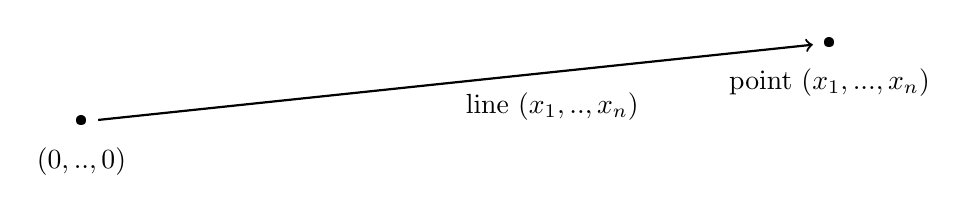
\begin{tikzpicture}[node distance=2cm]
		\node (A)[draw=none,label=below:{$(0,..,0)$}] at (0,0) {\textbullet};
		\node (B)[draw=none,label=below:{point $(x_1,...,x_n)$}] at (9.5,1) {\textbullet};
		
		\draw[thick, ->]
		(A) -- (B) 
		node[midway, below right] {line $(x_1,..,x_n)$};
	\end{tikzpicture}
	\caption{The correspondence between a line ``vector'' and a point ``vector''.}
\end{figure}

\begin{notation}
	Vectors are a very general notation of $n-tuples$. Depending on context, we use both of the following notations to denote the entries of $\vec{v}\in\reals^n$ \begin{itemize}
		\item ``Ordered sets'' $(v_1,...,v_n)$, suitable dealing with points (and other geometric objects). It also looks cleaner when writing inline.
		\item ``Column vectors'' $\begin{bmatrix}
			v_1\\.\\.\\.\\v_n
		\end{bmatrix}$ when the ordered sets are complicated to read, and when working with matrix algebra.
	\end{itemize}
\end{notation}
\subsection{Operation with lines}
We need to translate a few more things from euclidean geometry.

\proposition{
Let $\mathbf{x}, \mathbf{y}, \mathbf{z} \in \mathbb{R}^n$, then \[
	\overrightarrow{\mathbf{xy}}+\overrightarrow{\mathbf{yz}}=\overrightarrow{\mathbf{xz}},
\]
where $(a_1,...,a_n)+(b_1,...,b_n)\defeq(a_1+b_1,..., a_n+b_n)$.
}
\begin{proof}
	\begin{align*}
		\overrightarrow{\mathbf{xy}}+\overrightarrow{\mathbf{yz}}&=(y_1-x_1,..., y_1-x_n)+(z_1-y_1,..., z_1-y_n)\\
		&=(y_1-x_1+z_1-y_1, ... ,y_n-x_n+z_n-y_n)\\
		&= (z_1-x_1, ...,z_n-x_n)\\
		&= \overrightarrow{\mathbf{xz}}
	\end{align*}
\end{proof}
\

Geometrically, this means if you connect $\mathbf{x}$ to $\mathbf{y}$ to $\mathbf{z}$, the overall ``direction of travel" you make is $\mathbf{x}$ to $\mathbf{z}$. This gives us a natural extension for addition of vectors by considering each entry. Similarly for scaling vectors, we just scale the entries along each dimension.

 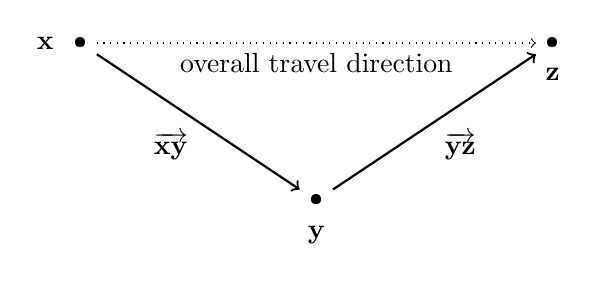
\begin{tikzpicture}[node distance=2cm]
 	\node (A)[draw=none,label=left:$\mathbf{x}$] at (0,0) {\textbullet};
 	\node (B)[draw=none,label=below:$\mathbf{y}$] at (3,-2) {\textbullet};
 	\node (C)[draw=none,label=below:$\mathbf{z}$] at (6,0) {\textbullet};
 
 	\draw[thick, ->]
 	(A) -- (B)
 	node[midway, below left]{$\overrightarrow{\mathbf{xy}}$};
 	\draw[thick, ->]
 	(B) -- (C)
 	node[midway, below right]{$\overrightarrow{\mathbf{yz}}$};
 	
 	\draw[dotted,->]
 	(A)--(C)
 	node[midway, below] {overall travel direction};
 	
 \end{tikzpicture}\ \\

\definition{Addition and scaling of vectors}{
	Let $\vec{a},\vec{b}$ be two vectors in $\mathbb{R}^n$. We define the sum/difference of $\vec{a}$ and $\vec{b}$ \[
		\vec{a}+\vec{b} \defeq (a_1+b_1,...,a_n+b_n), \quad \vec{a}-\vec{b} \defeq (a_1-b_1,...,a_n-b_n)
	\] and the scaling of $\vec{a}$ by a real number $c\in \mathbb{R}$ \[
		c\vec{a} \defeq (c a_1, c a_2,... ,c a_n).
	\]
}
\begin{remark}
	Here we use the term ``vectors", as we can in essence add points and lines together. How does one make sense of adding a line to a point? We can view this as translating the point along the path of the line, for instance, let us translate the point $(1,2)$ $3$ units in the first coordinate and $-1$ units in the second coordinate. This will give us $(4,1)$.
	
	\begin{figure}[h]
		\centering
		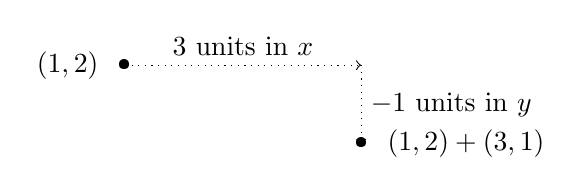
\begin{tikzpicture}[node distance=2cm]
			\node (A)[draw=none,label=left:{$(1,2)$}] at (1,2) {\textbullet};
			\node (y)[draw=none, label=right:{$(1,2)+(3,1)$}] at (4,1){\textbullet};
			\draw[->,dotted]
			(1,2)--(4,2)
			node [midway, above]{$3$ units in $x$};
			
			\draw[->, dotted]
			(4,2)--(4,1) node [midway,right]{$-1$ units in $y$};
		\end{tikzpicture}
	\end{figure}
\end{remark}

This way, we can write the line from $\vec{x}$ to $\vec{y}$ as $\vec{y}-\vec{x}$. The proof is a computational exercise. \\ 
\begin{notation}
	We now transferred for talking about points and the lines between points to addition. Therefore, we can overload the notation for points and lines as a vector $\vec{v}$, keeping in mind that they have the same arithmetic structure.
\end{notation}


In fact, most of our intuition for the real numbers translates to $\mathbb{R}$. For formality, we will list them here; in practice, we (almost always) take these properties for granted.
\proposition[vectorspace]{
	Let $\vec{u},\vec{v},\vec{w} \in \mathbb{R}^n$, and $a,b \in \mathbb{R}$. Then the following hold:
	\begin{itemize}
		\item \textit{(Associativity)} $(\vec{u}+\vec{v})+\vec{w} = \vec{u}+(\vec{v}+\vec{w})$.
		\item \textit{(Commutativity)} $\vec{u}+\vec{v} = \vec{v}+\vec{u}$.
		\item \textit{(Identity)} The zero vector $\vec{0}\defeq (0,0,...,0)\in\reals$ satisfies $\vec{v}+\vec{0}=\vec{v}$.
		\item \textit{(Inverse)} The inverse of $\vec{v}$, $-\vec{v}\defeq(-v_1,...,-v_n)$ satisfies $\vec{v}+(-\vec{v})=\vec{0}$.
		\item \textit{(Scalar multiplication)} $a(b\vec{v})=(ab)\vec{v}$.
		\item \textit{(Scalar Identity)} $1\vec{v}=\vec{v}$.
		\item \textit{(Distributivity 1)}  $a(\vec{u}+\vec{v})=a\vec{u}+a\vec{v}$.
		\item \textit{(Distributivity 2)}  $(a+b)\vec{v}=a\vec{v}+b\vec{v}$.
	\end{itemize}
} 
\begin{remark}
	All of these have good geometric intuition behind. For instance, the zero vector $\vec{0}$ is the ``don't move" vector, corresponding to the point at the origin, or the ``too short to be a line''. The inverse of $\overrightarrow{\mathbf{xy}}$ is $\overrightarrow{\mathbf{yx}}$, where you go back from $\mathbf{x}$ to $\mathbf{y}$. \begin{tikzpicture}
		
	\end{tikzpicture}
\end{remark}
\begin{remark}
	These $8$ conditions are the axioms of a vector space. Later in the course, we will generalize the notion of vectors in $\reals^n$ to other spaces (playing fields).
\end{remark}
\proposition{
	Lines are translation invariant. That is, for every $\vec{x},\vec{y},\vec{v}\in\mathbb{R}^n$, then the 
	line from $\vec{x}$ to $\vec{y}$ is the same as the line from $\vec{x}+\vec{v}$ to $\vec{y}+\vec{v}$.
}
Let us illustrate what this statement is trying to convey. We have two points $\vec{x}$, $\vec{y}$; now we translate each of these points by $\vec{v}$, and we want the line between the points to be preserved under this translation.\\
\begin{tikzpicture}
	\node (X)[draw=none,label=left:$\vec{x}$] at (0,0) {\textbullet};
	\node (Y)[draw=none,label=below:$\vec{y}$] at (5,-1) {\textbullet};
	\node (XT)[draw=none,label=below:$\vec{x}+\vec{v}$] at (-2,-2) {\textbullet};
	\node (YT)[draw=none,label=below:$\vec{y}+\vec{v}$] at (3,-3) {\textbullet};
	
	\draw[->,thick] 
	(X)--(Y)
	node (a)[midway, above right] {$\vec{y}-\vec{x}$};
	
	\draw[->,dotted] 
	(X)--(XT)
	node[midway, above left] {$\vec{v}$};
	
	\draw[->,dotted] 
	(Y)--(YT)
	node[midway, above left] {$\vec{v}$};
	
	
	\draw[->,color=blue] 
	(XT)--(YT)
	node[midway, below left] {?};
\end{tikzpicture} \ \\
The proof is one line: $(\vec{y}+\vec{v}) - (\vec{y}+\vec{v}) = \vec{y}-\vec{x} +\vec{v}-\vec{v}=\vec{y}-\vec{x}$. However, an immediate consequence of this is that we can ``transport'' vectors in space without distorting the vector. Colloquially, \textit{5 miles South} to you describes the same direction and length as \textit{5 miles South} to a person a few feet away. This justifies the way we visualize the correspondence between points and vectors - we ``transport'' the vectors to start from the origin $(0,...,0)$, and the end describes the point.

\begin{remark}
	Translation (and scaling) invariance is a property of Euclidean geometry. There are some exotic geometry systems that distort distance and direction through translation and scaling. One such example is the Poincar\'e metric.
\end{remark}
Another notion we can carry from Euclidean geometry is parallel lines. Here we not only define what it means for two vectors to be parallel (never touching), we also give a definition for two vectors to be parallel but point in opposite directions.
\definition{Parallel and Antiparallel Vectors}{
	Let non-zero vectors $\vec{v},\vec{w}\in\reals^n$.
	We say that $\vec{v}$ and $\vec{w}$ are \textbf{parallel} if there is some $c>0$ such that $\vec{v}=c\vec{w}$. We say that $\vec{v}$ and $\vec{w}$ are \textbf{antiparallel} if there is some $c<0$ such that $\vec{v}=c\vec{w}$.
}
\example{
	Find an expression for the points on the (infinite) line passing through $P(1,1,0)$ and $Q(0,2,2)$.
}
Let $M$ be a point on the line $\overrightarrow{PQ}$, then $\overrightarrow{PM}$ is parallel to $\overrightarrow{PQ}$ (or $M=P$). Either way, we would have some $c\in\reals$ such that \[
\overrightarrow{PM}=c\overrightarrow{PQ}.
\]
Indeed, we can confirm that any point represented as $P+c\overrightarrow{PQ}$ will be on the line, as $c\overrightarrow{PQ}$ is parallel to $\overrightarrow{PQ}$. One exception is to check for when $c=0$, but we already know $P$ is on the line.
We thus have an expression for the line to be \[
	(1,1,0) + c(-1,1,2)
\]
for all $c\in\reals$. Another way to put it, the line is the \textbf{image} of the function $f(c) = (1,1,0) + c(-1,1,2)$ on $\reals$.
\begin{remark}
	This form of representing a line is known as a \textbf{parametric representation} or a \textbf{parametrization} of the line. We will give a more concrete definition of parametrization when we move beyond straight lines to ``curvy'' curves and surfaces in \ref{noideayet}.
\end{remark}
\begin{remark}
	Using the parametric representation for a line $l(t) = (P_1,P_2,...,P_n)+ t(v_1,v_2,...,v_n)$, we can take slices/cross sections across each of the $j$-th coordinates, and get \[
	x_j = P_j+tv_j \implies t = \frac{x_j-P_j}{v_j}
	\] 
	is the equation of a line in 2d. $P_j, v_j$ are fixed, viewing in the variables $y=x_j, x=t$, this is the equation of a line with y-intercept $x_j$ and slope $v_j$. Setting the values of t for all slices to be equal, \[
	t= \frac{x_1-P_1}{v_1}=\frac{x_2-P_2}{v_2}=...=\frac{x_j-P_j}{v_j}=...=\frac{x_n-P_n}{v_n}
	\]
	This form is known as the \textbf{symmetric equations} of a line.
\end{remark}

\example{
	Find an expression for the points on the line connecting \textbf{between} $P(1,1,0)$ to $Q(0,2,2)$.
}
This will be a segment of the line from the previous example, so the answer would be the same expression, but we limit the domain of $f$ to be an interval on $\reals$. Let us examine what $f$ does to a few values of $c$.
\renewcommand{\arraystretch}{1.5}
\begin{center}
	\begin{tabular}{|c|c c c c c|} 
		\hline
		c & very negative & $c=0$ & $c=1/2$& $c=1$ & very positive \\ 
		\hline
		f(c) & very off the segment & $P$ & midpoint of $\overline{PQ}$& $Q$ & very off the segment \\ 
		\hline
	\end{tabular}
\end{center}
As we move from very negative $c$ to very positive $c$, we start very away from the line segment, reach $P$ at $c=0$, $Q$ at $c=1$, then move away from the line segment. 
Indeed the values $(1,1,0) + c(-1,1,2)$ will be on the line segment for $c\in[0,1]$.

%
Finally, the nice algebraic properties for adding and scaling vectors gives us a natural way to understand these vectors as a sum of $n$ component vectors, one for each dimension. These \textit{special} vectors deserve a name.
\definition{Standard Basis Vectors and Vector Decomposition}{
	We denote in $\reals^n$, the \textbf{standard basis vectors} \begin{align*}
		\vec{e}_1 &\defeq (1,0,0,...,0,0,0),\\
		\vec{e}_2 &\defeq (0,1,0,...,0,0,0),\\
		\vec{e}_{n-1}&\defeq (0,0,0,...,0,1,0),\\
		\vec{e}_n&\defeq(0,0,0,...,0,0,1),
	\end{align*}
	so that $\vec{v}=\sum_{i=1}^n v_i \vec{e}_i$.
	In $\reals^3$, we sometimes write \[
		\vec{i}\defeq \vec{e}_1, \quad \vec{j}\defeq \vec{e}_2,\quad \vec{k}\defeq\vec{e}_3
	\]to accommodate the physicists.
}\ \\
\exercises
\begin{exerciselist}
	\item Compute $5\vec{v}-2\vec{w}$ and $-3\vec{w}$ for the following pairs of vectors: \begin{enumerate}[label=(\alph*)]
		\item $\vec{v}=2\vec{i}+3\vec{j}$, $\vec{w}=4\vec{i}-9\vec{j}$
		\item $\vec{v}=(1,2,-1)$, $\vec{w}=(2,-1,0)$
		\item $\vec{v}=-2\vec{e}_3+4\vec{e}_5$, $\vec{w}=\vec{e}_1 -4\vec{e}_5$
		\item $\vec{v}=(\cos t, \sin t)$, $\vec{w}=(\cos t)\vec{e}_2 - (\sin t) \vec{e}_1$
	\end{enumerate}
	
	\item Find parametric equations that describe the line that \begin{enumerate}[label=(\alph*)]
		\item passes through $(1,2,3)$ and $(4,-1,2)$
		\item passes through $(0,-2,3)$ and $(1,2,3)$
	\end{enumerate}
\end{exerciselist}
\section{Length, angles and projections}
\definition{Magnitude}{
Let $\vec{v}\in\reals^n$. The magnitude of $\vec{v}$ is denoted \[
|\vec{v}| \defeq \sqrt{v_1^2 + v_2 ^2+ ... v_n^2}.
\]
}
We build intuition through the lower dimensional cases.
In $\reals^2$, let us consider the point $(4,3)$.\\
\begin{wrapfigure}{r}{0.3\textwidth}
	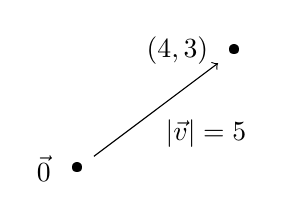
\begin{tikzpicture}
		\node (X)[draw=none,label=left:{$\vec{0}$}] at (0,0) {\textbullet};
		\node (Y)[draw=none,label=left:{$(4,3)$}] at (2,1.5) {\textbullet};
		\draw[->]
		(X)--(Y)
		node [midway, below right] {$|\vec{v}|=5$};
	\end{tikzpicture}
\end{wrapfigure}

The magnitude of this vector is $\sqrt{3^2+4^2}=5$. If this sounds very familiar, it is because this is indeed an application of Pythagorean theorem. In 3-dimensions, this still applies - take $\vec{x}=(a,b,c)$, we can traverse in each coordinate to apply Pythagorean theorem twice.

\usetikzlibrary {3d}

\begin{figure}[h]
	\centering
	\begin{subfigure}{0.3\textwidth}
		\centering
		\begin{tikzpicture}
			
			\draw[->](0,0,0) -- (xyz cylindrical cs:radius=3);
			\node at (3.5,0,0){$x_1$};
			\draw[->] (0,0,0) -- (xyz cylindrical cs:radius=3,angle=90);
			\node at (0,3.5,0){$x_2$};
			\draw[->] (0,0,0) -- (xyz cylindrical cs:z=3);
			\node at (0,0,3.5){$x_3$};
			\draw[->,dotted,thick,color=red] (0,0,0) -- (2,0,0)
			node[midway,below]{a};
			\draw[->,dotted,thick,color=red] (2,0,0) -- (2,3,0) node[midway,right]{b};
			\draw[->,dotted,thick,color=red] (2,3,0) -- (2,3,1)
			node[midway,above]{c};
			\draw[->,color=blue] 
			(0,0,0) -- (2,3,1)
			node[midway, below]{$\vec{x}$};
		\end{tikzpicture}
		\caption{$\vec{x}=(a,b,c)$.}
	\end{subfigure}
	\begin{subfigure}{0.3\textwidth}
		\centering
		\begin{tikzpicture}
			
			\draw[->](0,0,0) -- (xyz cylindrical cs:radius=3);
			\node at (3.5,0,0){$x_1$};
			\draw[->] (0,0,0) -- (xyz cylindrical cs:radius=3,angle=90);
			\node at (0,3.5,0){$x_2$};
			\draw[->] (0,0,0) -- (xyz cylindrical cs:z=3);
			\node at (0,0,3.5){$x_3$};
			\draw[->,dotted,thick,color=red] (0,0,0) -- (2,0,0)
			node[midway,below]{a};
			\draw[->,dotted,thick,color=red] (2,0,0) -- (2,3,0) node[midway,right]{b};
			\draw[->,color=brown] 
			(0,0,0) -- (2,3,0)
			node[midway, left]{$\sqrt{a^2+b^2}$};
			
		\end{tikzpicture}
		\caption{Pyth. thm on $a,b$.}
	\end{subfigure}
	\begin{subfigure}{0.3\textwidth}
		\centering
		\begin{tikzpicture}
			[z={(10:10mm)},x={(-45:5mm)}]
			
			\draw[->](0,0,0) -- (3,0,0);
			\node at (3.5,0,0){$x_1$};
			\draw[->] (0,0,0) -- (0,3,0);
			\node at (0,3.5,0){$x_2$};
			\draw[->] (0,0,0) -- (0,0,-3);
			\node at (0,0,-3.5){$x_3$};
			\draw[->,color=brown] 
			(0,0,0) -- (2,3,0)
			node[midway, right]{$\sqrt{a^2+b^2}$};
			
			\draw[->,dotted,thick,color=red] (2,3,0) -- (2,3,-1) node[midway, above]{c};
			\draw[->,color=blue] 
			(0,0,0) -- (2,3,-1)
			node[midway, left]{$\sqrt{a^2+b^2+c^2}$};
			
		\end{tikzpicture}
		\caption{Reapply Pyth. thm.}
	\end{subfigure}
	
\end{figure}\ \\

\proposition{
	Let $\vec{v} \in \reals^n, a\in\reals$. Then \[
	|a\vec{v}| = |a||\vec{v}|.
	\]
}\ \\
\definition{Unit vector}{
	Let $\vec{v}\in\reals^n$. We call $\vec{v}$ a \textbf{unit vector} if $|\vec{v}|=1$.
}
\proposition{
	Let $\vec{v}\in\reals^n$ be non-zero. Then there is a unique unit vector $|\vec{w}|=1$ such that $\vec{v}$ is parallel to $\vec{w}$.
}
\begin{proof}
	If $|\vec{w}|=1, c>0$ and $c\vec{w}=\vec{v}$, it must be that \[
		c = |c||\vec{w}| = |c\vec{w}| = |\vec{v}|,
	\]
	and \[
		\vec{w} = \frac{1}{c}(c\vec{w}) = \frac{1}{|vec{v}|}\vec{v}.
	\] This shows uniqueness - there is no other possible candidate except for this vector. Now we can confirm the vector $\frac{1}{|\vec{v}|}\vec{v}$ is a unit vector and is parallel to $\vec{v}$, so there exists a unique unit vector that satisfies the properties.
	\\
\end{proof}
We have now transported the notions of length and scaling into the coordinate system, and this allows us to make ``measurements'' such as angles and area.

\subsection{The Dot Product}
\example{
Let points A=$(5,8)$, B=$(-2, 7)$, O=$(4,5)$. Find the angle $\angle AOB$.
}
To solve this using only information about the lengths, recall the Law of Cosines:

\theorem{Law of Cosines}{
For any triangle 
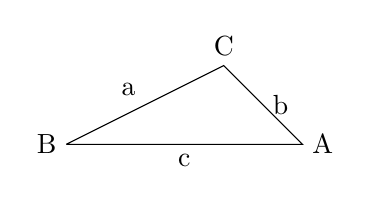
\begin{tikzpicture}
	
	\draw (0,0) node [left] {B}--(2,1) node [above]{C} node [midway, above left]{a}--(3,0) node [right]{A} node [midway, right]{b}--(0,0)node [midway, below]{c};
	%pic["$\alpha$",draw=orange,<->,angle eccentricity=1.2,angle radius=1cm] {angle=(0,0)--(2,1)--(3,0)};
\end{tikzpicture},
\[
	c^2 = a^2+b^2 - 2 a b \cos(\angle BCA).
\]
}

We now apply the Law of Cosines to $\triangle AOB$, so that\[
	|\overrightarrow{AO}|^2  +|\overrightarrow{OB}|^2- 2 |\overrightarrow{AO}| |\overrightarrow{OB} \ |\cos(\angle AOB) = |\overrightarrow{AB}|^2.
\]
Plugging in the values, we solve 
\begin{align*}
		((4-5)^2 + (5-8)^2) + ((-2-4)^2+(7-5)^2) - 2 \sqrt{(4-5)^2 + (5-8)^2} \\ \times \sqrt{(-2-4)^2+(7-5)^2} \cos(\angle AOB) = ((-2-5)^2+(7-8)^2).
\end{align*}
Simplifying, we get\[
	50 - 2 \sqrt{10} \sqrt{40} \cos(\angle AOB) = 50 \implies \cos(\angle AOB) = 0.
\]
So the angle is $\pi/2$.

\example{
	Find a closed form formula for the cosine of an angle formed by two vectors $\vec{v},\vec{w} \in\reals^n$.
}
Let the angle formed be $\theta$. Using the intuition from 2-D space, we can form a triangle (in a very complex n-dimensional space). We write the Law of Cosine in terms of vectors
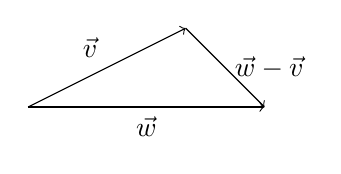
\begin{tikzpicture}
	
	\draw [->](0,0) -- (2,1) node [midway, above left]{$\vec{v}$};
	\draw [->](0,0)--(3,0) node [midway, below]{$\vec{w}$};
	\draw [->](2,1)--(3,0)node [midway, right]{$\vec{w}-\vec{v}$};
	%pic["$\alpha$",draw=orange,<->,angle eccentricity=1.2,angle radius=1cm] {angle=(0,0)--(2,1)--(3,0)};
\end{tikzpicture}
 \[
|\vec{v}|^2+|\vec{w}|^2-2|\vec{v}||\vec{w}|= |\vec{w}-\vec{v}|^2.
\]
This expands to \begin{align*}
	\sum_{i=1}^{n} v_i^2 + \sum_{j=1}^{n} w_j^2  - 2 \sqrt{\sum_{i=1}^{n} v_i^2}\sqrt{\sum_{j=1}^{n} w_j^2} \ \cos(\theta) =
	\sum_{i=1}^n (w_i-v_i)^2.
\end{align*}
Rearranging $(a-b)^2 = a^2+b^2-2ab$,
\[
2 \sqrt{\sum_{i=1}^{n} v_i^2}\sqrt{\sum_{j=1}^{n} w_j^2} \ \cos(\theta) = \sum_{i=1}^n 2 w_i v_i 
\]
so \[
\cos(\theta) = \frac{\sum_{i=1}^n w_i v_i }{\sqrt{\sum_{i=1}^{n} v_i^2}\sqrt{\sum_{j=1}^{n} w_j^2}}.
\]
\definition{Dot Product}{
	Let $\vec{v},\vec{w}\in\reals^n$, the \textbf{dot product} between $\vec{v}$ and $\vec{w}$ is \[
		\vec{v} \cdot \vec{w} \defeq \sum_{i=1}^n v_i w_i. 
	\]
}
\proposition{
Let $\vec{v}\in\reals^n$, then $|\vec{v}|^2 = \vec{v}\cdot\vec{v}$.
}
\proposition[1.22]{
	Let $\vec{u},\vec{v},\vec{w}\in\reals^n$, $c\in\reals$. The dot product satisfies the following properties:
	\begin{itemize}
		\item \textit{(Symmetry)} $\vec{v}\cdot\vec{w}=\vec{w}\cdot\vec{v}$.
		\item \textit{(Linearity 1)} $(c\vec{v})\cdot\vec{w} = c (\vec{v}\cdot\vec{w}) \textrm{(}= \vec{v}\cdot(c\vec{w})\textrm{  by symmetry)}$.
		\item \textit{(Linearity 2)} $(\vec{v}+\vec{u})\cdot\vec{w} = \vec{v}\cdot\vec{w}+\vec{u}\cdot\vec{w}$.
		\item \textit{(Positive definiteness)} $\vec{v} \cdot\vec{v}\geq0$, with equality if and only if $\vec{v}=\vec{0}$.
	\end{itemize}
}
\begin{proof}
	Here is the proof for the last property. The rest are left as an exercise We have $\vec{v}\cdot\vec{v} = |\vec{v}|^2\geq=0$, and if $\vec{v}\cdot\vec{v}=0$, for all $1\leq\j\leq n$, $v_j^2 \leq \sum_{i=1}^{n} v_i^2 = \vec{v}\cdot\vec{v}\leq0$, so $v_j=0$. This means $\vec{v}=\vec{0}$.
\end{proof}
\corollary[dotproduct]{
	
	\begin{enumerate}
		\item $
		|\vec{v}-\vec{w}|^2 = |\vec{v}|^2 + |\vec{w}|^2 - 2 \vec{v}\cdot\vec{w}.
		$
		\item In lower dimensions $\reals^2, \reals^3$ If $\vec{v},\vec{w}\neq \vec{0}$, the angle between $\vec{v}$ and $\vec{w}$ is\[
		\cos^{-1}\left(\frac{\vec{v}\cdot\vec{w}}{|\vec{v}||\vec{w}|}\right).
		\]
		In particular, the angle is $\pi/2$ when $\vec{v}\cdot\vec{w}=0$. 
		\item $|\vec{v}\cdot\vec{w}|\leq |\vec{v}||\vec{w}|.$
	\end{enumerate}
}

\theorem[cauchyschwarz]{Cauchy-Schwarz inequality}{
Let $\vec{v},\vec{u}\in\reals^n$. Then \[
	|\vec{v}\cdot\vec{u}|\leq |\vec{u}||\vec{v}|.
\]
}
The proof is in one of the exercises at the end of this chapter. \\
The dot product allows us to make sense of ``angles'' in higher dimensions, so we can generalize the notion of two vectors ``perpendicular'' to each other.
\definition{Orthogonality}{
Let $\vec{v},\vec{w}\in\reals^n$. We say $\vec{v}$ and $\vec{w}$ are \textbf{orthogonal} to each other if $\vec{v}\cdot\vec{w}=0$.
}

\example[1.26]{
	Find all vectors $\vec{v}\in\reals^3$ such that $\vec{v}\cdot(-3\vec{i}+2\vec{j}+6\vec{k}) =49$. Sketch the locus of corresponding points in $\reals^3$.
}

\label{plane_projection}
The condition expands to \begin{align*}
	-3v_1+2v_2+6v_3 &= 49 \\
	\implies v_3 &= \frac{49+3v_1 - 2v_2}{6}  
\end{align*}
so that the set of all vectors is \[
	\left\{s \vec{i}+t \vec{j}+\left(\frac{49+3s - 2t}{6}\right) \vec{k} | s,t\in\reals\right\}.
\]
To plot this in 3D space, notice that this describes the equation of a plane $z={(49+3x-2y)}/{6}$. We pick any three points (of course we want those that are easy to calculate) $(0,0,49/6)$, $(0,49/12,0)$, $(-49/18,0,0)$.
\iffalse
\begin{figure}
	\centering

	\subfloat%[\centering label 1]
	{{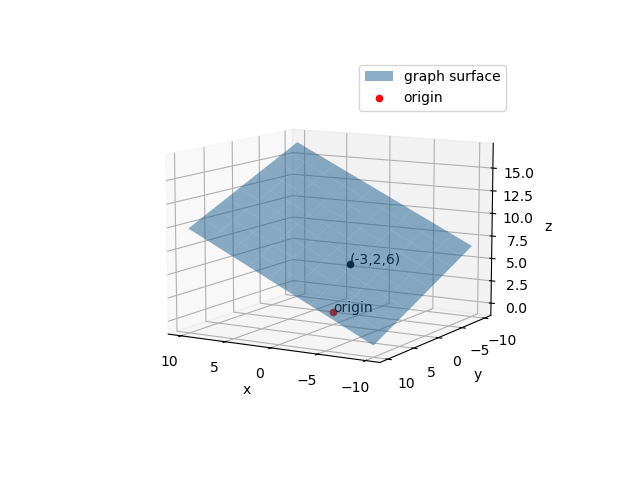
\includegraphics[width=7cm]{coordinate_geometry/plane1.png} }}%
	\qquad
	\subfloat%[\centering label 2]
	{{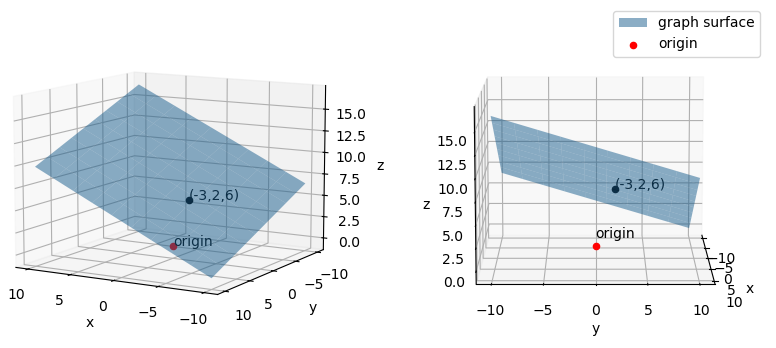
\includegraphics[width=7cm]{coordinate_geometry/plane2.png} }}%
	\caption{Two views of the plane}
\end{figure}
\fi
\begin{lstlisting}[language=Python]
	def function_to_plot(X,Y):
	return (49+3*X-2*Y)/6
	#create figure
	fig=plt.figure(figsize=(10,8))
	ax = fig.add_subplot(projection='3d')
	ax.view_init(elev=10, azim=120) #change view 1  
	#ax.view_init(elev=10, azim=0) #change view 2
	X,Y=np.meshgrid(np.linspace(-10,10,10), np.linspace(-10,10,10))
	Z=function_to_plot(X,Y)
	surface=ax.plot_surface(X, Y, Z, alpha=0.5,
	label='graph surface')
	ax.set_xlabel('x')
	ax.set_ylabel('y')
	ax.set_zlabel('z')
	#plot the curve and the cross section to integrate
	ax.scatter(0,0,0,color='red',label='origin')
	ax.text(0,0,0,'origin')
	ax.scatter(-3,2,6,color='black')
	ax.text(-3,2,6,'(-3,2,6)')
	plt.legend()
	plt.show()
\end{lstlisting}

\begin{figure}[h]
	\centering
	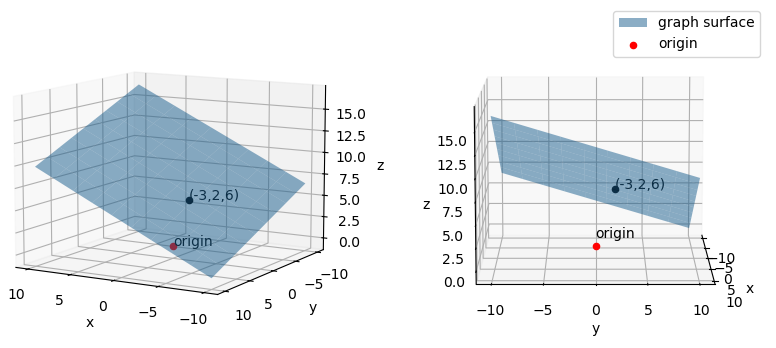
\includegraphics[width=\textwidth]{coordinate_geometry/plane2.png}
	\caption{Two views of the plane}
\end{figure}\ \\

Interestingly, we see that $(-3,2,6)$ - the point corresponding to our vector - is a point on the plane!
\begin{remark}
	The form \[
		\left\{s \vec{i}+t \vec{j}+\left(\frac{49+3s - 2t}{6}\right) \vec{k} | s,t\in\reals\right\}
	\] is a \textbf{parametrization} of the plane described by $-3x+2y+6z=49$, viewing this as a function $\reals^2\to\reals^3$.
\end{remark}
\subsection{Projection}
\definition{Projection}{
Let $\vec{v},\vec{w}\in\reals^n$, $\vec{v}\neq\vec{0}$, and $c\in\reals$, such that $\vec{v}\cdot(\vec{w}-c\vec{v})=0$ (or equivalently, $\vec{w}-c\vec{v}$ orthogonal to $\vec{v}$). 

We say that $c\vec{v}\defeq \textrm{Proj}_{\vec{v}} (\vec{w})$ is the \textbf{vector projection of $\vec{w}$ on $\vec{v}$}.

}\ \\

\iffalse
\begin{notation}
	The vector projection ``encodes'' information about the scalar projection. Therefore, if we do not specify scalar or vector, assume are talking about vector projections.
\end{notation}
\fi
To build intuition, it is always helpful to start with lower dimensions. We take a plane through $\vec{v}$ and $\vec{w}$. Looking at this slice, we can work in 2D.


We see that $c\vec{v}$ is the the point on the extension of $\vec{v}$ such that it is closest to the point $\vec{w}$. To geometrically show this idea, we draw a circle centered at $\vec{w}$ with radius $|\vec{w}-c\vec{v}|$. The line generated by $\vec{v}$ is tangent to this circle, so the contact point at $c\vec{v}$ is indeed the closest point to $\vec{w}$. 
\usetikzlibrary{angles} 
\begin{figure}[h]
	\centering
	\begin{subfigure}{0.4\textwidth}
		\centering
		\begin{tikzpicture}
			\node (x) at (0,0){};
			\node (y) at (5,0){};
			\node (z) at (5,-2){};
			\draw[->,thick]
			(0,0) -- (3,0) node [midway, above] {$\vec{v}$};
			\draw[->,thick]
			(0,0) -- (5,-2) node[midway, below left]{$\vec{w}$};
			\draw[dotted]
			(5,-2) -- (5,0) node [midway, right] {$\vec{w}-c\vec{v}$};
			\draw[->,red,dotted] 
			(0,0)--(5,0) node[midway, above right]{$\textrm{Proj}_{\vec{v}}(\vec{w}) = c\vec{v}$};
			
			\pic [draw, angle eccentricity=0.5]{right angle=x--y--z};
		\end{tikzpicture}
	\end{subfigure}
	\begin{subfigure}{0.4\textwidth}
		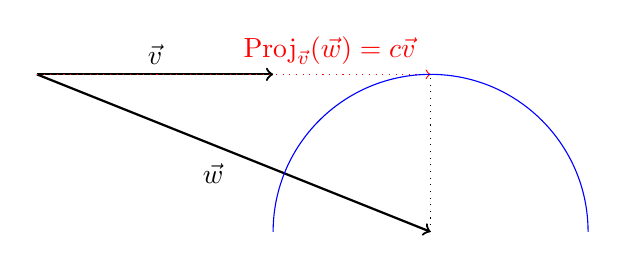
\begin{tikzpicture}
			\node (x) at (0,0){};
			\node (y) at (5,0){};
			\node (z) at (5,-2){};
			\draw[->,thick]
			(0,0) -- (3,0) node [midway, above] {$\vec{v}$};
			\draw[->,thick]
			(0,0) -- (5,-2) node[midway, below left]{$\vec{w}$};
			\draw[dotted]
			(5,-2) -- (5,0);
			\draw[->,red,dotted] 
			(0,0)--(5,0) node[midway, above right]{$\textrm{Proj}_{\vec{v}}(\vec{w}) = c\vec{v}$};
			
			\draw [blue](7,-2)arc (0:180:2);
		
		\end{tikzpicture}
	\end{subfigure}
\end{figure}
	
	
	

We also see from this geometric construction that 1) the projection $c\vec{v}$ is unique thus well defined, 2) $c|\vec{v}|=|\vec{w}|\cos \theta$

\proposition{
The projection is unique and is given by \[
	\textrm{Proj}_{\vec{v}}(\vec{w}) = \frac{\cos \theta |\vec{w}|}{|\vec{v}|} = \frac{\vec{v}\cdot\vec{w}}{|\vec{v}|^2} = \left(\frac{\vec{v}\cdot\vec{w}}{\vec{v}\cdot\vec{v}}\right)\vec{v}.
\]

}
This is the first time we show that something is unique. The standard argument goes as follows: Suppose another object $a'$ satisfies all the properties you want for $a$. Then you can show $a=a'$, meaning every object that satisfies the properties is $a$, or equivalently, $a$ is unique. 

So what happens if we pick two points $P$, $P'$ on $\vec{v}$ such that both make a right angle when connected to $\vec{w}$? We would have constructed a triangle $\triangle PP'\vec{w}$ with two right angles!
\begin{proof}
	Let $c, c'\in\reals$ such that $\vec{p}_1=c\vec{v}$ and $\vec{p}_2=c'\vec{v}$ are both satisfy the definition of $\textrm{Proj}_{\vec{v}}({\vec{w}})$. We want to show that $c=c'$, so we consider $\vec{u}=(c-c')\vec{v}$, the line between the two projections.\\
	By corollary \ref{cor:dotproduct}, we have two equations \begin{align*}
	|\vec{w}-\vec{p}_1|^2&=|\vec{w}-\vec{p}_2|^2+|\vec{u}|^2 \\	
	|\vec{w}-\vec{p}_2|^2&=|\vec{w}-\vec{p}_1|^2+|\vec{u}|^2 
	\end{align*}
	We can solve for $|\vec{u}|=0$, and by positive definiteness, $\vec{u}=\vec{0}$ and $c-c' = |\vec{u}|/|\vec{v}| =0$.\\
	To show our formula for projection works, we can just compute that \[
	\vec{v} \cdot \left(\vec{w}-\left(\frac{\vec{v}\cdot{\vec{w}}}{\vec{v}\cdot\vec{v}}\right)\vec{v}\right)=\vec{v}\cdot\vec{w} -\left(\frac{\vec{v}\cdot\vec{w}}{\vec{v}\cdot\vec{v}}\right)(\vec{v}\cdot\vec{v})=0.
	\]
\end{proof}
\exercises
\begin{exerciselist}
	\item Determine if the following pairs of vectors are orthogonal: \begin{enumerate}[label=(\alph*)]
		\item $3\vec{e}_1+4\vec{e}_2$, $-4\vec{e}_1+3\vec{e}_2$
		\item $(4,-1,2)$, $(3,0,-6)$
		\item $3\vec{i}-2\vec{j}$, $-2\vec{i}-4\vec{k}$
		\item $\vec{e}_1 + 3\vec{e}_3 + 5\vec{e}_5+ ...+(2k-1)\vec{e}_{2k-1}$, $2\vec{e}_2+4\vec{e}_4+...+(2k)\vec{e}_{2k}$
	\end{enumerate}
	\item Refer to the plane in Example \ref{ex:1.26}. Show that $\textrm{Proj}_{-3\vec{i}+2\vec{j}+6\vec{k}}(\vec{v})$ is the same for any vector $\vec{v}$ such that $\vec{v}\cdot(-3\vec{i}+2\vec{j}+6\vec{k}) =49$, and compute this projection.
	\item \textit{(Geometry of a methane molecule)} Place four points $P(0,0,0)$, $Q(1,1,0)$, $R(1,0,1)$, $S(0,1,1)$ in $\reals^3$. \begin{enumerate}[label=(\alph*)]
		\item Compute the distance between any two points of $PQRS$ and show that all $6$ pairs are the same. This means that $PQRS$ forms a regular tetrahedron.
		\item  Verify that the geometric center of the tetrahedron $O(1/2, 1/2, 1/2)$ is equidistant to all of the vertices of the tetrahedron.
		\item Compute the angle between two edges of the tetrahedron, rounded to $2$ decimal places. By symmetry, you only have to compute one angle.
		\item Compute the angle $\angle POQ$, rounded to $2$ decimal places. Does this angle remind you of something from Chemistry?
	\end{enumerate}
\end{exerciselist}
\section{Cross Product}
\definition{Cross Product}{
Let $\vec{v},\vec{w}\in\reals^3$, we define the \textbf{cross product} of $\vec{v}$ and $\vec{w}$ to be \[
	\vec{v}\times\vec{w}\defeq \begin{bmatrix}
		v_2w_3-v_3w_2\\
		v_3w_1 - v_1w_3\\
		v_1w_2 - v_2w_1\\
	\end{bmatrix}.
\]
}
\begin{remark}
	Later on, we will introduce determinants of a matrix. The cross product can be understood as the determinant of the `matrix'\[
	\begin{bmatrix}
		\vec{i} & v_1 & w_1 \\
		\vec{j} & v_2 & w_2 \\
		\vec{k} & v_3 & w_3
	\end{bmatrix}.
	\]
\end{remark}
This definition seems a bit unmotivating, so let us work through some examples.
\example{
	Compute the $9$ cross products for each pair of the standard basis vectors in $\reals^3$.
}
With some (heavy) computation, we find
\begin{align*}
	\vec{i}\times\vec{i}&=\vec{0} \quad& \vec{i}\times\vec{j}&=\vec{k} \quad& \vec{i}\times\vec{k}&=-\vec{j} \\
	\vec{j}\times\vec{i}&=-\vec{k} \quad& \vec{j}\times\vec{j}&=\vec{0} \quad& \vec{j}\times\vec{k}&=\vec{i}\\
	\vec{k}\times\vec{i}&=\vec{j} \quad& \vec{k}\times\vec{j}&=-\vec{i} \quad& \vec{k}\times\vec{k}&=\vec{0}
\end{align*}
Importantly, the cross product is \textbf{antisymmetric}, meaning $\vec{v}\times\vec{w}=-\vec{w}\times\vec{v}$. You can see special cases with the standard basis from above and confirm the general case in an exercise.
\example{
	Compute $\vec{v} \cdot (\vec{v}\times\vec{w})$ and $\vec{w}\cdot (\vec{v}\times\vec{w})$.
}
Again with some heavy computation,
\begin{align*}
	\vec{v} \cdot (\vec{v}\times\vec{w}) &= \begin{bmatrix}
		v_1 \\v_2\\v_3
	\end{bmatrix}\cdot\begin{bmatrix}
	v_2w_3-v_3w_2\\
	v_3w_1 - v_1w_3\\
	v_1w_2 - v_2w_1\\
	\end{bmatrix} \\
	&= \color{red}v_1v_2w_3\color{black}-\color{black}v_1v_3w_2\color{black}+\color{blue}v_2v_3w_1\color{black}-\color{red}v_2v_1w_3\color{black}+\color{black}v_3v_1w_2\color{black}-\color{blue}v_3v_2w_1\\
	&=0,\\
	\vec{w} \cdot (\vec{v}\times\vec{w}) &= \begin{bmatrix}
		w_1 \\w_2\\w_3
	\end{bmatrix}\cdot\begin{bmatrix}
		v_2w_3-v_3w_2\\
		v_3w_1 - v_1w_3\\
		v_1w_2 - v_2w_1\\
	\end{bmatrix} \\
	&= \color{red}w_1v_2w_3\color{black}-\color{black}w_1v_3w_2\color{black}+\color{black}w_2v_3w_1\color{black}-\color{blue}w_2v_1w_3\color{black}+\color{blue}w_3v_1w_2\color{black}-\color{red}w_3v_2w_1\\
	&=0.\\
\end{align*}
Which means $\vec{v}\times\vec{w}$ is orthogonal to $\vec{v}$ and $\vec{w}$!

\example{
	Compute $|\vec{v}\times\vec{w}|^2 + (\vec{v}\cdot\vec{w})^2$.
}
We have
\begin{align*}
|\vec{v}\times\vec{w}|^2 + (\vec{v}\cdot\vec{w})^2 =&
(v_2w_3-v_3w_2)^2 +(v_3w_1 - v_1w_3)^2 + (v_1w_2 - v_2w_1)^2 
\\ &+ 
(v_1w_1 + v_2w_2 + v_3w_3)^2\\
=& (v_1w_1)^2+(v_1w_2)^2+(v_1w_3)^2\\&+(v_2w_1)^2+(v_2w_2)^2+(v_2w_3)^2\\&+(v_3w_1)^2+(v_3w_2)^2+(v_3w_3)^2\\
=&(v_1^2 + v_2^2+v_3^2)(w_1^2+w_2^2+w_3^3)\\
=&|\vec{v}|^2|\vec{w}|^2.
\end{align*}
Now we substitute $\vec{v}\cdot\vec{w}=|\vec{v}||\vec{w}|\cos\theta$, we get \[
	|\vec{v}\times\vec{w}|=|\vec{v}||\vec{w}|\sqrt{1-\cos^2\theta} = |\vec{v}||\vec{w}|\sin\theta.
\]
Where we know $\sin \theta \geq 0$ as $\theta$ is between $0$ and $\pi$.

The value $|\vec{v}||\vec{w}|\sin\theta$ has a nice geometric meaning. It is the area spanned by the vectors $\vec{v}$ and $\vec{w}$.\ \\
\usetikzlibrary{angles} 
\begin{figure}[h]%{r}{0.4\textwidth}
	\centering
\begin{tikzpicture}
	\node (X)[draw=none] at (0,0) {};
	\node (Y)[draw=none] at (5,0) {};
	\node (XT)[draw=none] at (-2,-2) {};
	\node (YT)[draw=none] at (3,-2) {};
	
	\draw[->,thick] 
	(0,0)--(5,0)
	node (a)[midway, above left] {$\vec{w}$};
	
	\draw[->,thick] 
	(0,0)--(-2,-2)
	node[midway, above left] {$\vec{v}$};
	
	\draw[->,dotted] 
	(5,0)--(3,-2)
	node[midway, above left] {$\vec{v}$};
	
	
	\draw[->,dotted] 
	(-2,-2)--(3,-2)
	node[midway, below left] {$\vec{w}$};
	\pic [pic text=$\theta$,draw,angle eccentricity=1.5] {angle = XT--X--Y};
	\draw[dotted]
	(0,0)--(-2,0) node (O) {}--(-2,-2)
	node [midway, left]{$|\vec{v}|\sin\theta$};
	\pic [draw, angle eccentricity=0.5]{right angle=XT--O--X};
\end{tikzpicture}
\caption {The area of a parallelogram formed by these vectors is the magnitude of the vector $\vec{v}\times|\vec{w}|$}
\end{figure} \ \\
\proposition{
	The direction of $\vec{v}\times\vec{w}$ is determined by the \textbf{right-hand rule} as follows:
	\begin{quotation}
		Using the right hand, align the index finger with the direction $\vec{v}$, and the middle finger with the direction of $\vec{w}$. Extend the thumb so that it is perpendicular to both the index finger and the middle finger. The thumb is pointing in the direction of $\vec{v}\times \vec{w}$.
	\end{quotation}
}
This is a byproduct of the convention we use. In $\reals^3$ we use what is known as a right-handed coordinate system - the vectors $\vec{i}$, $\vec{j}$, and $\vec{k}$ align with the first three fingers of the right hand respectively. If we used a left-handed coordinate system, the rule would be left-handed instead. 
\begin{figure}[h]
	\centering
	\begin{subfigure}[l]{0.4\textwidth}
		\centering
		\begin{tikzpicture}
			
			\draw[->](0,0,0) -- (xyz cylindrical cs:radius=3);
			\node at (3.5,0,0){$x_2$};
			\draw[->] (0,0,0) -- (xyz cylindrical cs:radius=3,angle=90);
			\node at (0,3.5,0){$x_3$};
			\draw[->] (0,0,0) -- (xyz cylindrical cs:z=3);
			\node at (0,0,3.5){$x_1$};
		\end{tikzpicture}
		\caption {Right handed coordinate system}
	\end{subfigure}
	\begin{subfigure}[r]{0.4\textwidth}
		\centering
			\begin{tikzpicture}
			\draw[->](0,0,0) -- (xyz cylindrical cs:radius=3, angle=180);
			\node at (-3.5,0,0){$x_2$};
			\draw[->] (0,0,0) -- (xyz cylindrical cs:radius=3,angle=90);
			\node at (0,3.5,0){$x_3$};
			\draw[->] (0,0,0) -- (xyz cylindrical cs:z=3);
			\node at (0,0,3.5){$x_1$};
		\end{tikzpicture}
		\caption {Left handed coordinate system}
	\end{subfigure}
\end{figure}
We now have a few properties about the cross product from our computation, the first you will verify on your own:
\proposition{
	Let $\vec{v},\vec{w},\vec{u}\in\reals^n$, then 
	\begin{itemize}
		\item \textit{(distributivity)} $\vec{v}\times(\vec{u}+\vec{w})=\vec{v}\times\vec{u}+\vec{v}\times\vec{w}$ and $(\vec{v}+\vec{u})\times\vec{w}=\vec{v}\times\vec{w}+\vec{v}\times\vec{u}$.
		\item \textit{(anti-symmetry)} $\vec{v}\times\vec{w}=-\vec{w}\times\vec{v}$.
		\item $\vec{v}\times\vec{w}$ is orthogonal (perpendicular in 3D space) to $\vec{v}$ and $\vec{w}$.
		
		\item The magnitude $|\vec{v}\times\vec{w}|$ is given by $|\vec{v}||\vec{w}|\sin\theta$, with $\theta$ being the angle between $\vec{v}$ and $\vec{w}$, so \begin{enumerate}[label=(\roman*)]
			\item The magnitude $|\vec{v}\times\vec{w}|$ also corresponds to the area of the parallelogram formed by $\vec{v}$ and $\vec{w}$.
			\item If $\vec{v}$ and $\vec{w}$ are parallel or antiparallel, $\vec{v}\times\vec{w}=\vec{0}$.
		\end{enumerate}		
	\end{itemize}
}
\begin{remark}
	Using distributivity of the cross product, you only need to memorize the cross product of the basis vectors, and write $\vec{v}\times\vec{w}=\sum_{i=1}^{3}\sum_{j=1}^3v_iw_i (\vec{e}_i\times\vec{e}_j)$.
\end{remark}
\subsection{Triple products}
\example{
	Find the volume of the parallelepiped formed from $\vec{v}=\begin{bmatrix}
	0\\1\\1
	\end{bmatrix}$, $\vec{w}=\begin{bmatrix}
	1\\1\\0
	\end{bmatrix}$, $\vec{u}=\begin{bmatrix}
	1\\0\\1
	\end{bmatrix}$.
}

%\usetikzlibrary{perspective}

The parallelepiped is a generalization of a parallelogram to higher dimensions. Using combinations of $\vec{v},\vec{w},\vec{u}$, you can make the frame of a 3d solid. As in the figure on the left, edges of the same color correspond to the same vector (and thus parallel). The volume of this solid is still $base \times height$, where the base is a 2D parallelogram formed by two vectors and the height is determined by third vector. We make an arbitrary decision and set the base to be $\vec{v}$ and $\vec{w}$. (setting any two vectors would give the same result in the end!) The area of this base is given by the cross product
\[
	\vec{A}=\vec{v}\times\vec{w} = \begin{bmatrix}
		-1\\1\\-1
	\end{bmatrix}.
\]\ \\

Now we can determine the height of the paralellepiped from $\vec{u}$. We want to isolate the component of $\vec{u}$ that is orthogonal to the base. Equivalently, we want to find the component of $\vec{u}$ that is pointing in the direction of $\vec{A}$, a vector that is orthogonal to both $\vec{v}$ and $\vec{w}$!\ \\
\begin{figure}[h]%{r}{\textwidth}
	\centering
	\begin{subfigure}{0.4\textwidth}
		\centering
		\begin{tikzpicture}
			[z={(10:10mm)},x={(-45:5mm)}]
			
			\draw[->](0,0,0) -- (xyz cylindrical cs:radius=3);
			\node at (3.5,0,0){$x_1$};
			\draw[->] (0,0,0) -- (xyz cylindrical cs:radius=3,angle=90);
			\node at (0,3.5,0){$x_2$};
			\draw[->] (0,0,0) -- (xyz cylindrical cs:z=3);
			\node at (0,0,3.5){$x_3$};
			\draw[->,color=red] 
			(0,0,0)--(0,1,1)
			node[midway, below] {\color{red}$\vec{v}$};
			\draw[->,color=blue] 
			(0,0,0)--(1,0,1)
			node[midway,below]{\color{blue}$\vec{u}$};
			\draw[->,color=green] 
			(0,0,0)--(1,1,0)
			node[midway, left]{\color{green}$\vec{w}$};
			
			\draw[->,color=red] 
			(1,0,1)--(1,1,2);
			
			\draw[->,color=green] 
			(1,1,2)--(2,2,2);
			\draw[->,color=red] 
			(1,1,0)--(1,2,1);
			\draw[->,color=green] 
			(1,0,1)--(2,1,1);
			\draw[->,color=red] (2,1,1)--(2,2,2);
			\draw[->,color=green] 
			(0,1,1)--(1,2,1);
			
			\draw[->,color=blue] 
			(1,1,0)--(2,1,1);
			
			\draw[->,color=blue] 
			(1,2,1)--(2,2,2);
			\draw[->,color=blue]
			(0,1,1)--(1,1,2);
		\end{tikzpicture}
		\caption{The parallelepiped, draw in an optical illusion fashion.}
	\end{subfigure}
	\begin{subfigure}{0.4\textwidth}
		\centering
		\begin{tikzpicture}
			[z={(10:10mm)},x={(-45:5mm)}]
			
			\draw[->](0,0,0) -- (xyz cylindrical cs:radius=3);
			\node at (3.5,0,0){$x_1$};
			\draw[->] (0,0,0) -- (xyz cylindrical cs:radius=3,angle=90);
			\node at (0,3.5,0){$x_2$};
			\draw[->] (0,0,0) -- (xyz cylindrical cs:z=3);
			\node at (0,0,3.5){$x_3$};
			\draw[->,color=red] 
			(0,0,0)--(0,1,1)
			node[midway, below] {\color{red}$\vec{v}$};
			\draw[->,color=blue] 
			(0,0,0)--(1,0,1)
			node[midway,below]{\color{blue}$\vec{u}$};
			\draw[->,color=green] 
			(0,0,0)--(1,1,0)
			node[midway, left]{\color{green}$\vec{w}$};
			\draw[->,dotted,thick]
			(0,0,0)--(-1,1,-1)
			node[midway,left]{$\vec{A}$};
			\draw[->,color=red] 
			(1,1,0)--(1,2,1);
			\draw[->,color=green] 
			(0,1,1)--(1,2,1);
			
		\end{tikzpicture}
		\caption{We want to get the projection of $\vec{u}$ on $\vec{A}$.}
	\end{subfigure}
\end{figure}\ \\
The volume is thus \[
	|\textrm{Proj}_{\vec{A}}(\vec{u})||\vec{v}|=\left|\frac{\vec{u}\cdot\vec{A}}{|\vec{A}|^2}\right|\times |\vec{A}| \times|\vec{A}| = |\vec{u}\cdot\vec{A}| = 2.
\]\ \\

\proposition{
The volume of the parallelpiped formed from $\vec{v},\vec{w},\vec{u}$ is \[
|(\vec{v}\times\vec{w})\cdot{\vec{u}}|
\]
}\ \\

\begin{remark}
	This is also the expression of the (absolute value of) determinant of \[
	\begin{bmatrix}
		\vec{v}&\vec{w}&\vec{u}
	\end{bmatrix}
	\]
	where $\vec{v},\vec{w},\vec{u}$ are written as column vectors.
	Using properties of the determinant (later chapters), you can show cycling the three vectors does not change the volume. (i.e. you can calculate using what order of the three vectors you want)
\end{remark}
	
\begin{remark}
	You may notice that the expression $(\vec{v}\times\vec{w})\cdot{\vec{u}}$ can take on negative volumes. In this case, the three vectors (taken in order) do not follow the right-hand rule. For instance, in the last example, $\vec{u}$ points in the `opposite' direction as $\vec{A}$.
\end{remark}
\exercises
\begin{exerciselist}
	\item Find $\vec{v}\times\vec{w}$ for the following: \begin{enumerate}[label=(\alph*)]
		\item $\vec{v}=(4,-2,0)$, $\vec{w}=(2,1,-1)$
		\item $\vec{v}=(3,3,3)$, $\vec{w}=(4,-3,2)$
		\item $\vec{v}=2\vec{i}+3\vec{j}+4\vec{k}$, $\vec{w}=\vec{i}-3\vec{j}+4\vec{k}$
	\end{enumerate}
	\item Find the areas for the following shapes:\begin{enumerate}[label=(\alph*)]
		\item The parallelogram with vertices $P(0,0,0), Q(1,1,0),R(1,2,1),S(0,1,1)$.
		\item The triangle with vertices $A(1,9,3),B(-2,3,0),C(3,-5,3)$.
	\end{enumerate}
	\item Find the volume of the parallelepiped formed from the vectors $\vec{v}=(1,1,0),\vec{w}(0,2,-2),\vec{u}=(1,0,3)$.
	\item A triangular kite has vertices $P(0,0,10),Q(2,1,10),S(0,3,12)$ and is displaced by the wind at a velocity of $(20\vec{i}+6\vec{j}+4\vec{k})/s$\begin{enumerate}[label=(\alph*)]
		\item Find the area of the kite.
		\item After 1/2 seconds, find the volume of the space swept by the kite. (leave the answers in $[units]^3$)
	\end{enumerate}
\end{exerciselist}

\section{Applications - Geometry of lines and planes}
\definition{Relations between lines}{
For two (infinitely extending) lines in $\reals^n$ parametrized in $s$ and $t$ respectively as $l_1=P + t\vec{v}$, $l_2=Q+s\vec{w}$, we say the lines are \begin{itemize}
	\item \textbf{Parallel}, if the $\vec{v}$ and $\vec{w}$ are parallel or antiparallel.
	\item \textbf{Intersecting}, if $l_1$ and $l_2$ exactly one point on both $l_1$ and $l_2$.
	\item \textbf{Skew}, if $l_1$ and $l_2$ are not parallel/antiparallel or intersecting.
\end{itemize}
}
\begin{remark}
	Lines do not have direction, so there usually is no need to distinguish between parallel and antiparallel lines. One may extend the definition of antiparallel to lines from $\vec{v}$ and $\vec{w}$.
\end{remark}
\proposition{
Determination of parallel lines are independent of parametrization. Concretely, 
\begin{quotation}
Let $P_1+t_1\vec{v}_1$ and $P_2+t_2\vec{v}_2$ be two parametrizations of $l_1$, $Q_1+s_1\vec{w}_1$, $Q_2+s_2\vec{w}_2$ be two parametrizations of $l_2$. If $\vec{v}_1 =c_1\vec{w}_1$ for some $c_1\in\reals$, then $\vec{v}_2=c_2\vec{w}_2$ for some (possibly different )$c_2\in\reals$.
\end{quotation}
}
The proof is not very enlightening. However, the result of this guarantees that our definition of parallel lines is precise.
\begin{proof}
	The idea is to show that $\vec{v}_1$ is a scalar multiple of $\vec{v}_2$, and by the same logic $\vec{w}_1$ is a scalar multiple of $\vec{w}_2$. Since all vectors are non-zero in the parametrization, we will get the result of $\vec{v}_2$ a scalar multiple of $\vec{w}_2$. 
	
	To show $\vec{v}_1=k\vec{v}_2$ for some $k$, we can pick two distinct points $A,B$ on $l_1$. From the parametriation we can get $\alpha_1,\alpha_2,\beta_1,\beta_2\in\reals$ such that $P_1+\alpha_1\vec{v}_1=A=P_2+\alpha_2\vec{v}_2$ and $P_1+\beta_1\vec{v}_1=B=P_2+\beta_2\vec{v}_2$. Therefore we get the vector \begin{align*}
		\overrightarrow{AB}&=(\beta_1-\alpha_1)\vec{v}_1,\\
		\overrightarrow{AB}&=(\beta_2-\alpha_2)\vec{v}_2.
	\end{align*}
	As we picked distinct points $A$ and $B$, we can conclude $\overrightarrow{AB}\neq\vec{0}$ and thus $\beta_1-\alpha_1\neq0,\beta_2-\alpha_2\neq0$, so that \[
		\vec{v}_1= \frac{\beta_2-\alpha_2}{\beta_1-\alpha_1}\vec{v}_2.
	\]
\end{proof}
\example{
Determine whether the lines parametrized by $l_1(t)=(1,2,1)+t(1,3,-2)$ and $l_2(t)=(3,1,0)+t(-2,-6,4)$ are parallel, intersecting, or skew. Confirm that $l_1$ and $l_2$ describe two different lines. 
}
We notice that $-2\times(1,3,-2)=(-2,-6,4)$, so these lines are parallel. To confirm that these two lines are not the same, we notice that $(1,2,1)$ is a point on $l_1$, but if we attempt to solve\[
(1,2,1)=l_2(t)=(3,1,0)+t(-2,-6,-4) \implies (-2,1,1)=t(-2,-6,-4) 
\]
which no $t$ can solve! Specifically, the first coordinate forces $t=1$ and the second coordinate forces $t=-6$. 
\example{
Determine whether the lines parametrized by $l_1(t)=(1,2,1)+t(1,3,-2)$ and $l_2(t)=(0,3,9)+t(0,2,3)$ are parallel, intersecting, or skew.
}
$(1,3,2)$ is not a multiple of $(0,2,3)$, so the lines are not parallel. We might be tempted to solve for $l_1(t)=l_2(t)$ to check for intersection, but this misses a lot of cases! We need to compare all the points of $l_1$ with all the points of $l_2$, so we need two independent variables to describe where we are on each of the lines. That is, we solve for $s,t$ in $l_1(t)=l_2(s)$,
\begin{align*}
	(1,2,1)+t(1,3,-2) &=(0,3,9)+s(0,2,3)\\
	\implies (t+1,3t+2,-2t+1) &= (0,2s+3,3s+9)\\
	\implies t=-1 \textrm{ and } &3t+2=2s+3 \textrm{ and } -2t+1=3s+9
\end{align*}
$t=-1, s=-2$ solves this system of equations. We can plug in $t$ and $s$ in our original parametrization to find $(0,1,3)$ is indeed a point on both $l_1$ and $l_2$. We would have missed this if we set $l_1(t)=l_2(t)$! 
\example{
	Determine whether the lines parametrized by $l_1(t)=(1,2,1)+t(1,3,-2)$ and $l_2(t)=(0,3,8)+t(0,2,3)$ are parallel, intersecting, or skew.
}
We repeat the same process as above to see that the lines are not parallel and solve for 
\begin{align*}
	(1,2,1)+t(1,3,-2) &=(0,3,8)+s(0,2,3)\\
	\implies (t+1,3t+2,-2t+1) &= (0,2s+3,3s+8)\\
	\implies t=-1 \textrm{ and }& 3t+2=2s+3 \textrm{ and } -2t+1=3s+8
\end{align*}
This time, we do not have a solution - the first two equations forces $t=-1, s=-2$, and this does not solve the third. We therefore do not have a point of intersection, and the lines are skew.
\example{
	Determine if $P(5,6,9), Q(7,9,15), R(13,18,33)$ are \textbf{colinear} i.e. if they lie on the same line. 
}
With the machinery we have built up, there are multiple ways to check if $P,Q,R$ form a straight line. Here are a few ideas:\begin{enumerate}
	\item Check that $\overrightarrow{PQ}$ is parallel/antiparallel to $\overrightarrow{PR}$. Because the lines defined by $\overline{PQ}$ and $\overline{PR}$ are parallel and share a same point $P$, they are the same line.
	\item Use the dot product to calculate the angle $\angle PQR=\pi$.
	\item Use the cross product to calculate that $\overrightarrow{PQ}\times\overrightarrow{PR}=\vec{0}$. This means the triangle with vertices $P,Q,R$ has no area and thus is a degenerate triangle.

\end{enumerate}
\definition{Characterization of Planes}{
	In euclidean geometry, planes can be characterized by any of the following ways: \begin{itemize}
		\item For \textbf{any three non-colinear points} $P_1,P_2,P_3$, there is a unique plane passing through $P_1,P_2,P_3$.
		\item For \textbf{any pair of intersecting lines}, there is a unique plane that contains both.
		\item For \textbf{a line $l$ and a point $P$}, there is a unique plane that contains $P$ and is perpendicular to $l$.
		\item For \textbf{a line $l$ and a point $P$ not on $l$}, there is a unique plane that contains both $l$ and $P$.
	\end{itemize}
}
\begin{remark}
	The third characterization is the hardest to visualize at first, but is also the easiest to describe with the analytical tools we have built towards. We can refer to Example \ref{ex:1.26}. The plane sketched is the unique plane that contains $(-3,2,6)$, such that each vector in the plane is orthogonal to $(-3,2,6)$, so the line parametrized by $l(t)=t(-3,2,6)$ is perpendicular to the plane at the point of intersection $(-3,2,6)$.
\end{remark}

\example[1.44]{
	In $\reals^3$, determine the equation of the plane that contains $P_0(x_0,y_0,z_0)$ and is perpendicular to the line parametrized by $l(t)=Q_0+t\vec{N}$, $\vec{N}=(a,b,c)$.
}
First we can exploit \textbf{translation invariance} of $\reals^3$ and move the line to $\tilde{l}=P_0 + t\vec{N}$. Because $l$ and $\tilde{l}$ are parallel, any line perpendicular to $l$ will also be perpendicular to $\tilde{l}$.\\
Then by the characterization of a plane, any $P$ on the plane satisfies the orthogonality relation $\overrightarrow{PP_0}\cdot\vec{N}=0$. Expanding this, we get the equation \[
a(x-x_0)+b(y-y_0)+c(z-z_0)=0 \implies ax+by+cz=ax_0+by_0+cz_0.
\]
\definition{Normal form of a plane}{
Let $a,b,c,d\in\reals$, with at least one of $a,b,c\neq0$. The equation of a plane in $\real^3$ written as \[
ax+by+cz=d
\]
is called a \textbf{normal form} of the equation of a plane.
}
\begin{remark}
	As all planes can be characterized this method, all equations of planes can be put in normal form.
\end{remark}
\begin{remark}
	The normal form of a plane is not unique. Pick your favorite non-zero number $\alpha$, the equation $\alpha ax+\alpha by+\alpha c_z=\alpha d$ describes the same plane.
\end{remark}
\theorem[normalvectorofplane]{Normal vectors of planes}{
When written in normal form, the plane is perpendicular to the vector $\vec{N}=(a,b,c)$. We call this vector $\vec{N}$ the \textbf{normal vector}.
}
We thus have a definition for two planes to be parallel.
\definition{Parallel planes}{
Two planes are \textbf{parallel} if the normal vectors are parallel.
}
A problem in the exercise will guide you through the proof of Theorem \ref{thm:normalvectorofplane}. The intuition behind the proof is the reverse direction of the equation $\overrightarrow{PP_0}\cdot\vec{N}=0$ we derived from the last example.\\
We will now apply this theorem in a few examples.
\example{
Find the equation of the plane that passes through the points $P(1,0,0),Q(0,1,0),R(0,0,1)$.
}
\textbf{Method 1:} One sees that (by coincidence) the sum of coordinates of each point are equal to $1$, so immediately writes down $x+y+z=1$. Despite being the fastest method, this is somewhat inconsistent.\\


\textbf{Method 2:} We set $ax+by+cz=d$ to be the equation, and plug in values for $P,Q,R$, giving the system of equations\begin{align*}
	a+0b+0c&=d \\ 0a+b+0c&=d \\ 0a+0b+c&=d 
\end{align*}
This is an \textbf{underdetermined system}, meaning there are fewer equations than unknowns. The best we can say is that $a=b=c=d$. However, setting $a=b=c=d=k$ works for all $k\neq 0$, further confirming that the normal form is not unique. This method is reasonably fast when the system of equations are simple. When there are more non-zero coefficients, solving the system takes more time.\\

\textbf{Method 3:} We can compute the direction of the normal vector $\vec{N}$ of this plane. By the characterization of planes, $\vec{N}$ is orthogonal to $\overrightarrow{PQ}$ and $\overrightarrow{PR}$, two vectors in the plane. We can thus write $\vec{N}$ as a multiple of the cross product \[
	\overrightarrow{PQ} \times \overrightarrow{PR} = \begin{bmatrix}
		-1\\1\\0
	\end{bmatrix} \times \begin{bmatrix}
	-1\\0\\1
	\end{bmatrix} = \begin{bmatrix}
	1\\1\\1
	\end{bmatrix}
\]. Using this normal vector (or any multiple of it) and applying the theorem, we get $x+y+z=d$, and substituting $P$ into the equation will give $x+y+z=1$. This method is more general and consistent, as the number of operations in a cross product is constant.

\example{
On the plane given by $ax+by+cz=d$, find the point on the plane that is closest to the origin.
}
\begin{wrapfigure}{r}{0.35\textwidth}
	\centering
	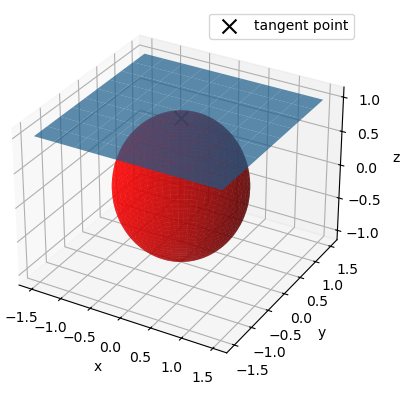
\includegraphics[width=0.3\textwidth]{coordinate_geometry/tangent.png}
	\caption{A toy example with the unit sphere of radius $1$ and the plane described by $z=1$.}
\end{wrapfigure}
Let $r$ be the distance, we draw a sphere centered at the origin with radius $r$. This sphere is thus tangent to the surface at one point, and the vector corresponding to this point will be perpendicular to the plane. By the theorem, we can denote the point $P(\alpha a, \alpha b, \alpha c)$, with $\alpha$ a constant to be determined. Substituting $P$ into the equation, \begin{align*}
	\alpha (a^2+b^2+c^2) = d \implies \alpha = \frac{d}{a^2+b^2+c^2}
\end{align*}
The closest distance from the origin is \[
|(\alpha a, \alpha b, \alpha c)| = |\alpha| \sqrt{a^2+b^2+c^2} = \left| \frac{d}{\sqrt{a^2+b^2+c^2}}\right| 
\]
at the point \[
\left(\frac{da}{\sqrt(a^2+b^2+c^2)},\frac{db}{\sqrt(a^2+b^2+c^2)},\frac{dc}{\sqrt(a^2+b^2+c^2)}\right)
\]\ \\
\subsection{Intersection of planes}
\example{
Find the intersection of the planes given by \begin{align*}
	6x+2y-z&=2\\
	\textrm{and } x-2y+3z&=5.
\end{align*}
}
\textbf{Method 1:} The line lies on the first plane, so is perpendicular to its normal vector $(6,-2,-1)$. The line also lies on the second plane, so is perpendicular to its normal vector $(1,-2,3)$. Using the cross product, the line should point in the direction of \[
\begin{bmatrix}
	6\\2\\-1
\end{bmatrix} \times\begin{bmatrix}
1\\-2\\3
\end{bmatrix}=\begin{bmatrix}
4\\-19 \\ -14
\end{bmatrix}
\]
Now we just need to find one point $P$ on the line of intersection, so that the parametric equation (in $t$) is $P+t(4,-19,-14)$.
We can impose an additional restriction that $x=0$ (or $y=0$ or $z=0$) and solve the simultaneous equations\begin{align*}
	2y-z&=2\\
	-2y+3z&=5.
\end{align*}
and get $(0,11/4,7/2)$ is a point on the intersection. The final parametric representation is $l(t)=(0,11/4,7/2)+t(4,-19,-14)$.

\textbf{Method 2:} We can solve the system of equations to find the line of intersection, and arrive at the set of symmetric equations. A similar method would be to solve for two points on the line of intersection, then get the parametric equation. This method will be introduced later\\
\exercises
\begin{exerciselist}
	\item Find parametric and symmetric equations for the line that \begin{enumerate}[label=(\alph*)]
		\item passes through $(0,0,0)$ and is parallel to $\vec{v}=3\vec{i}+4\vec{j}+5\vec{k}$
		\item passes through $(1,1)$ and is perpendicular to the line described by $y=3x+3$
		\item passes through $(0,1,2)$ and is perpendicular to plane with equation $3x+4y=2+z$
		\item passes through $(0,1,2)$ and is perpendicular to the yz-plane
		\item passes through $(1,3,0)$ and is parallel to the line with symmetric equations $x=y-1=(z-3)/2$
	\end{enumerate}
	\item Determine if these pair of lines are parallel, intersecting, or skew: \begin{enumerate}[label=(\alph*)]
		\item (As described by parametric equations) $l_1(t)=(1,-1,2)+t(2,1,1), l_2(t) = t(1,0,-1)$
		\item The line passing through $(3,1,3)$ and $(-2,-4,-5)$ and the line passing through $(1,3,5)$ and $(11,13,21)$.
	\end{enumerate}
	\item Determine if $P(3,1,2),Q(-1,0,2), R(11,3,2)$ are colinear.
	\item Find an equation for the plane \begin{enumerate}[label=(\alph*)]
		\item Containing $P(1,2,0)$ with normal vector $\vec{N}=2\vec{i}-\vec{j}+3\vec{k}$
		\item containing $P(2,4,5)$ with normal vector $\vec{N}=\vec{i}+3\vec{k}$
		\item containing $P(1,4,3)$ and perpendicular to the line given by the parametrization $r(t)=(1+t,2+4t,t)$
		\item containing the origin and parallel to the plane described by $3x+4y-6z=-1$
		\item containing the points $P(0,0,0),Q(1,-2,8),R(-2,-1,3)$
	\end{enumerate}
	\item Find the intersection of the planes with equations $2x+3y-z=1$ and $x-y-z=0$
	\item Find the angle between the normal vectors of the following planes: \begin{enumerate}[label=(\alph*)]
		\item the planes with equations $x+2y-z=2$ and $2x-y+3z=1$
		\item the plane with equation $2x+3y-6z=0$ and the plane containing the points $P(1,3,-2)$, $Q(5,1,3)$, $R(1,0,1)$
		\end{enumerate}
\end{exerciselist}

\section{End of Chapter Exercises}
\begin{exerciselist}
	\item Let $PQRS$ be a parallelogram. Show that $\overline{PR}$ and $\overline{QS}$ bisect each other i.e. intersect at their midpoints. 
	\item Complete the proof to Proposition \ref{1.22} - Show that the dot product is symmetric and linear. 
	\item Prove the \hyperref[thm:cauchyschwarz]{Cauchy-Schwarz inequality}. Here is a hint: Write $\vec{w} =  \textrm{Proj}_{\vec{v}}{\vec{w}} + (\vec{w}-\textrm{Proj}_{\vec{v}}{\vec{w}})$, and take the squared-magnitude on each side using the dot product.
	\item Prove or give a counterexample: The cross product is associative.
	\item Prove the following identity: $(\vec{a}\times\vec{b})\times\vec{c} = -(\vec{b}\cdot\vec{c})\vec{a}+(\vec{a}\cdot\vec{c})\vec{b}$.
	\item Show that the cross product satisfies the Jacobi identity: For any $\vec{a},\vec{b},\vec{c}\in \reals^3$, $(\vec{a}\times\vec{b})\times\vec{c} + (\vec{b}\times\vec{c})\times\vec{a} +(\vec{c}\times\vec{a})\times\vec{b} =\vec{0}$.
	\item On the plane given by $ax+by+cz=d$, show that the closest distance from $P(x_1,y_1,z_1)$ to the plane is given by $|ax_1+by_1+cz_1-d|/\sqrt{a^2+b^2+c^2}$. (Hint: Refer to Example \ref{ex:1.44})
	\item Define two lines in $\reals^3$ by the parametric equations \begin{align*}
		l_1(t) = \vec{r}_1 + t\vec{v}_1\\
		l_2(t)=\vec{r}_2+t\vec{v}_2
	\end{align*}
	We will derive a formula for the shortest distance between the two lines.
	\begin{enumerate}[label=(\alph*)]
		\item Consider the special case where the two lines are parallel. Construct two points $A$ and $B$ on $l_1$ and $l_2$ respectively. Find $B'$ Such that $\overrightarrow{AB'} = \textrm{Proj}_{\vec{v_1}}(\overrightarrow{AB})$. Argue that $B'$ is on the line $l_1$, and that the line $\overline{BB'}$ is perpendicular to $l_1$ and $l_2$. Conclude that the shortest distance between $l_1$ and $l_2$ is given by \[
			\sqrt{|\vec{r}_2-\vec{r}_1|^2 - \left(\frac{(\vec{r}_2-\vec{r_1})\cdot\vec{v}_1}{|\vec{v}_1|}\right)^2}
		\] 
		\item Now we can assume the lines are not parallel. Find a vector $\vec{N}$ that is perpendicular to both lines.
		\item (In your mind,) look in the direction of $\vec{N}$. $\vec{N}$ will now look like a dot. The lines will seem to overlap at points $A'$ and $B'$ respectively. Argue that $\overline{A'B'}$ is the shortest line from $l_1$ to $l_2$, and it is given by \[
			\overrightarrow{A'B'}=\textrm{Proj}_{\vec{N}}(\overrightarrow{AB})
		\], for any $A$ on $l_1$ and $B$ on $l_2$.
		\item Conclude that the shortest distance in this case is given by \[
			\left|\frac{(\vec{r}_2-\vec{r_1}) \cdot(\vec{v}_1\times\vec{v}_2)}{|\vec{v}_1\times\vec{v}_2|}\right|.
		\]
		\item Suppose $l_1$ and $l_2$ intersect at $P$. Verify that the formula evaluates to $0$, thus it gives a criterion to check if two lines intersect.
	\end{enumerate}
\end{exerciselist}

	
\end{document}